\chapter{AortaGeomRecon Research and Development}
This chapter will discuss about the research and development of the \progname{}. \\
AortaGeomRecon stands for Aorta Geometry Reconstruction. The main objective of this software is to semi-automatically build 3D geometry of the Aorta from the patient's chest ct scans.  The existing methods are often involved of extensive manual works with very complex software, with a minimum of 10 minutes of human operator, who is a medical domain expert. \\
The implementation till the date of this report can let the users who have the user characteristics described in SRS get the Aorta 3D geometry with only a few hyperparameters and 2 minutes of execution time. \\


\section{Existing Methods}
There are many segmentation software available to the users, we will discuss the two main methods on two softwares.


\begin{itemize}
\item ITK-Snap\\
ITK-Snap provides a segmentation method that first let user to select multiple voxels with a custom intial size and expanding size within any volume. We refer this method as ``bubble method''.\\
Through many iterations, the voxels expand to fill the entire volume, finally user will need to cut the extra part of the volume. \\
The advantages of the bubble method is that it guarantes to produce a correct the segmentation result. A medical domain expert can manually control the wanted area, and visually observing the segmentation result expanding, shrinking and the user can erase the unwanted part.

The disadvantages of this method is that the operations described above are complicated. Eeasier to say then do, an opeartor who has previous experience building the geometry with this method still needed 20 minutes of manual work building a new aorta geometry. ITK-Snap software can only read VTK file, therefore the chest CT scans are usually DICOM needed a manual conversion before using this software and its segmentation method.

\item 3D Slicer\\
3D Slicer is another well-known medical image processing software for academic. 3D Slicer provides multiple segmentation methods, and one of the quickiest and easiest to use is the intensity based segmentation.\\

This method first let user select a small area that belongs to the wanted area on a 2D plane (Axial, Sagittal, and ). 3D Slicer read the pixels' intensity of the surrounding area, and segment based on the intensity. Any pixels's intensity that are within the range will be segmented as the segmentation result. 

Like the bubble method, this method often reads extra volume, and requires user to cut the unwanted parts. A Youtube video shows an experience user who gets the aorta 3D geometry with 10 minutes of manual works.
\end{itemize}


\section{GitHub and Workflows}
This project uses GitHub for version control. \\
GitHub issues tracker use to keep track the items to work on throughout the development of the project\\
GitHub Project is used for dividing a large issue into smaller tasks, expected date of the completion. This is useful for project management.\\
GitHub Workflow is a great tool for Continuous Integration tests. \\
We uses GitHub Workflow for Linter and Continuous Integration tests. \\

\section{3D Slicer Extension Development}
The project has started with the a simple segmentation algoritm build on the jupyter notebook. When getting a new patient's data, the user will need to investigate the chest ct scans using another software (3D Slicer, ITK-Snap), in order to know the starting voxel and the size crop the volume, and get the index of the aorta seed. This Figure~\ref{fig_aorta_seed} shows an example of the aorta seeds.

\begin{figure}[ht]
    \centering
    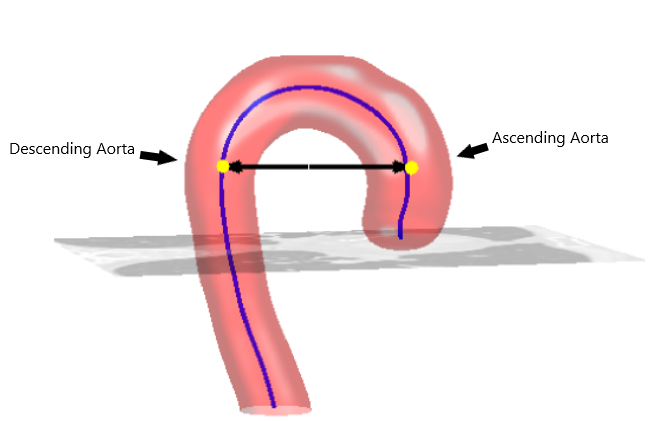
\includegraphics[width=0.6\textwidth]{figures/Sample/Aorta_seeds.png}
    \caption[Single Figure Environment Listed Title]{The aorta seeds}
    \label{fig_aorta_seed}
\end{figure}

In order to improve the usability of the \progname{} (reduce the amount of time for user inputs and execution), we implemented an extension module on 3D Slicer. 

3D Slicer provides 

\section{Segmentation Algorithm}

This is a sample chapter

If you need to use quotes, type it ``like this''.


\section{Referencing}
These are some sample references to GAMYGDALA~\citep{popescu2014gamygdala} from 
the \texttt{references.bib} file and state effects of 
cognition~\citep{hudlicka2002time} from the \texttt{references\_another.bib} 
file. These references are not in the same .bib file.
%
%\section{Figures}
%This is a single image figure (Figure~\ref{fig_singleenv}):
%
%\begin{figure}[ht]
%    \centering
%    
\includegraphics[width=0.6\textwidth]{figures/Sample/tumblr_static_eaceks0rfxsss8o4swscw40wo.jpg}
%    \caption[Single Figure Environment Listed Title]{This is a single figure 
%    environment}
%    \label{fig_singleenv}
%\end{figure}
%
%This is a multi-image figure with a top (Figure~\ref{fig_multienv_1}) and bottom (Figure~\ref{fig_multienv_2}) aligned subfigures:
%
%\begin{figure}[ht]
%	\centering
%	\begin{subfigure}[t]{\textwidth}
%		\centering
%		
%
\includegraphics[width=0.7\textwidth]{figures/Sample/tumblr_static_eaceks0rfxsss8o4swscw40wo.jpg}
%		\caption{Figure 1}
%		\label{fig_multienv_1}
%	\end{subfigure}
%	~
%	\begin{subfigure}[t]{\textwidth}
%		\centering
%		
%
\includegraphics[width=0.7\textwidth]{figures/Sample/tumblr_static_eaceks0rfxsss8o4swscw40wo.jpg}
%		\caption{Figure 2}
%		\label{fig_multienv_2}
%	\end{subfigure}
%	
%	\caption{A Multi-Figure Environment}
%	\label{fig_multienv}
%\end{figure}
%
%\section{Tables}
%
%Here is a sample table (Table~\ref{tab_sample}):
%
%	\begin{table}[ht]
%	\centering
%	\begin{tabular}{ m{0.2\textwidth} m {0.1\textwidth} m{0.15\textwidth} }
%		\toprule
%		A & $\longleftrightarrow$ & B \\
%		C & $\longleftrightarrow$ & D \\
%		\bottomrule	
%	\end{tabular}	
%	\caption{A sample table}	
%	\label{tab_sample}
%\end{table}
%
%\subsection{Long Tables}
%A sample long table is shown in Appendix~\ref{appendix_b}.
%
%\section{Equations}
%
%Here is a sample equation (Equation~\ref{eq_lineslope}):
%
%\begin{equation} \label{eq_lineslope}
%	y = mx + b
%\end{equation}